\documentclass{report}
\usepackage{graphicx} 
\usepackage{booktabs}
\usepackage{url}  
\begin{document}
\renewcommand\bibname{References}  

%include the title page
\begin{titlepage}
\begin{center}
\textup{\small {\bf A \\Seminar } \\ Report on}\\[0.2in]
% Title
\Large \textbf { Cache Memory }\\[0.5in]

        \vspace{.2in}

      \textbf {In Partial Fulfillment of Bachelor of Technology \\in\\ Computer Science and Engineering}\\[0.5in]
\normalsize Submitted by \\
\textbf{Dinesh Kumar Mali}

\vspace{1cm}
\normalsize Submitted To  \\
\textbf{Mr. Rajkumar Chaudhary}


\vspace{1cm}
Under the guidance of\\
{\textbf{Guide's name here}}\\[0.2in]


\vspace{2cm}
% Bottom of the page

\includegraphics[width=0.18\textwidth]{./Ecb_logo.png}\\[0.1in]
\large{\textbf{Department of Computer Science and Engineering}}\\
\normalsize
\textsc{\textbf{Government Engineering College Bikaner}}\\
\vspace{0.2cm}


\end{center}

\end{titlepage}


\pagenumbering{roman}
\begin{center}

\huge{\textbf{Department of Computer Science and Engineering}}\\[0.5cm]
\normalsize
\textsc{\textbf{Govt. Engineering College Bikaner}}\\[2.0cm]

\emph{\LARGE Certificate}\\[2.5cm]
\end{center}
\normalsize This is to certify that the Seminar Report entitle Cache Replacement Policies has been submitted by Mr. \textbf{Dinesh Kumar Mali}  in partial in fulfillment for the requirement of the degree of Bachelor of Technology, Final Year for the academic Session 2017-2018.
work as prescribed by Rajasthan Technical University, Kota.
\\[1.0cm]



\vfill


% Bottom of the page

       
        
\begin{flushleft}         
Dinesh Kumar Mali
\\14EEBCS021,
\\CSE,
\\dkmsn8@gmail.com ,
\\Govt. ECB, Bikaner
\end{flushleft}

\vspace{1cm}
\begin{flushleft}
Date:
\\Place: Bikaner
\end{flushleft}







\begin{center}
\huge{\textbf{Department of Computer Science and Engineering}}\\[0.5cm]
\normalsize
\textsc{\textbf{Govt. Engineering College Bikaner}}\\[2.0cm]



\emph{\LARGE Acknowledgement}\\[2.5cm]
\end{center}

\normalsize This is opportunity to express my heartfelt words for the people who were part of this seminar in numerous ways, people who gave me unending support right from beginning of the  seminar report.

\vspace{1cm}
I want to give sincere thanks to the principal, Prof. Dinesh Shringi, sir for his valuable support.
I extend my thanks to Mr. \textbf{Ranu Lal Chauhan}, HOD CSE Department for his cooperation and guidance.





\vfill


% Bottom of the page
\begin{flushright}
Yours Sincerely,
\\\textbf{Dinesh Kumar Mali}


\end{flushright}







\begin{abstract}
  In this Given Report of Seminar we are studying three Research Papers
Viz  \textit{The V-Way Cache : Demand-Based Associativity via Global Replacement}
  \cite{Qureshi2005TheVC}\textit{A Case for MLP-Aware Cache Replacement}\cite{Qureshi2006ACF} and \textit{Bank-aware Dynamic Cache Partitioning for Multicore Architectures} \cite{Kaseridis2009BankawareDC} .
The First Paper proposed the V way, set 
associative cache achieves an average miss rate reduction by 13 \% on sixteen benchmarks.The Second Paper proposed a framework for MLP-aware cache replacement by a run-time technique by calculating MLP-based cost for all and A low-overhead Hardware \emph{Sampling Based Adaptive replacement (SBAR)} to dynamically choose between MLP-aware and traditional replacement.
The third paper proposed a dynamic partitioning method based on realistic last level cache designs of \emph{CMP processors} it used a Cycle accurate ,Full system simulator based on and \emph{8-core DNCUA CMP system}.
\end{abstract}


\pagenumbering{roman} 
\tableofcontents
 \addcontentsline{toc}{chapter}{Certificate}
\setcounter{page}{1}
 \addcontentsline{toc}{chapter}{Acknowledgement}


\listoffigures
\listoftables
\newpage
\pagenumbering{arabic}

\chapter{The V-Way Cache }
\section{Introduction}
Cache hierarchies in CPU play A very important role in bridging
the gap between the processor speed and Memory Latency. As
processor speed increases and memory latency becomes more critical, intelligent design of secondary caches becomes very important.The performance of the cache directly depends on its success at storing data which will be used in future.In a set-associative cache, the number of entries to replacement policy is limited to numbers of ways.On a miss, a victim is identified from set of ways.The replacement policy could 
\vspace{.8cm}
select better victim by considering the global access history of each victim.
Inorder to achieve the lowest possible miss rate, a cache should be organized as fully associative with \emph{Beldays OPT} replacement policy but we know that  \emph{OPT} sees the future which we cant.The power, latency and hardware cost of fully-associative make it impractical and  \emph{OPT} is Impossible as we know that it needs Future knowledge we don't have.
Doubling the associativity to 16 ways this improves the miss rate, where making cache  fully-associative results in much more improvement.The fully-associative cache with 
\emph{OPT} even reduces the miss rate than \vspace{.8cm}a set-associative cache of double size.


A fully-associative cache has two advantages which are distinct over a set-associative cache:\emph{conflict -miss minimization } and \emph{global replacement}.There is an inverse relationship between the number of conflicts -misses in a cache and the associativity of cache. A fully set-associative cache always minimized conflict -misses by maximizing associativity. Also,as the associativity of cache increases, the scope of the information to perform replacement increase.

\begin{figure}[t]
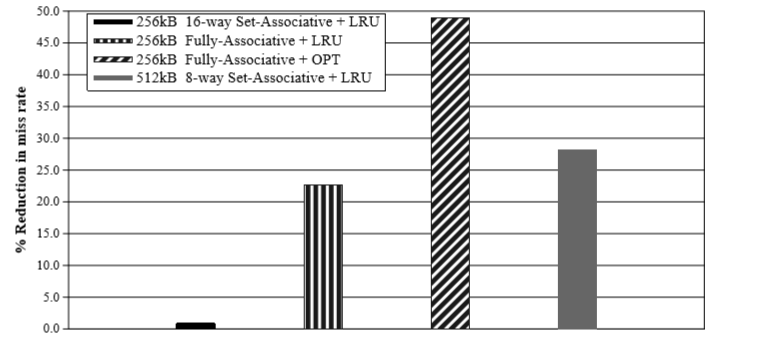
\includegraphics[width=1\textwidth]{./fig1}
\caption{Percent reduction in miss rate compared to a 256kB 8-way set-associative cache.}
\label{fig1}
\end{figure}


\vspace{5cm}
The Contribution of This paper works as follows :
\begin{enumerate}
\item They Proposed a novel mechanism to provide the benefit of global replacement while maintaining hit latency of set-associative cache. They call this \emph{Variable-Way} Set Associative or \emph{V-way Cache}.
\item For the V-way cache, They propose a practical global replacement policy based on the fact on access frequency called \emph{Resue Replacement}. Resue replacement performs perfectly than LRU policy at a fraction of hardware cost and complexity 

\end{enumerate}

\section{Motivation}
\subsection{Problem}

Memory accesses in basic purpose application are non-uniformly distributed across the sets in the cache.This in-uniform creates a heavy demand on some sets , which can cause conflict misses, while other sets remain underutilized.Victim cache are small,fully-set associative buffers that provide limited additional associativity for big utilized entries in a direct -mapped cache.
\vspace{.8cm}
With these Schemes, if the first attempt to access the cache results in a miss and hash function is changed.These techniques were proposed for first level direct -mapped cache, and their  effectiveness reduces as associativity increases due to inherent performance in increase associativity .
\subsection{Example}
the V-way Cache With example. Consider the four-way
set-associative cache shown in the figure \ref{fig2} .For simplicity, the cache contains only two sets: Set A and Set B. The data-store is shown as a linear array .The memory references in working set of X all map to set A, while x0 ,x1 etc are represented in the figure as 'x0', 'x1' etc.
\vspace{1cm}
\begin{figure}[h!]
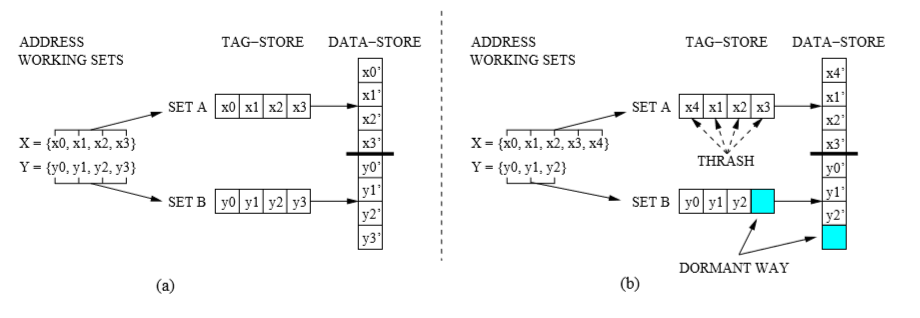
\includegraphics[width=1\textwidth]{./fig2}
\caption{ Traditional set-associative cache using local replacement.
}
\label{fig2}
\end{figure}

If cache accesses are totally uniform as in Figure 1.2(a),
the demand on Set A and B is equal and both halves of data-store. This is not a case in actual application.Due to variable demand on sets. In Figure 1.2(b), presumably at a different phase in the program, working set X increase by one and Y decreased by.
set A is unable accommodate all so resultinmg conflict misses and thrashing.Set B on the hand has a dormant way.A Basic Set-associative cache cannot adapt its associativity because lines in the data-store are statically mapped to entries in tag store.This static partitioning local replacement.When a cache miss occurs a victim is chosen within target set and corresponding entries in tag-store and data-store are replaced.

\subsection{Solution}
By increasing the number of tag-store entries relative to the data lines proved the flexibility to accommodate data cache lines on per set basis Figure 1.3(a) shows the same example from \ref{fig2}, here a number of tag store is doubled. By doing this the typically 2-3\%  \vspace{.8cm}to the overall storage requirement of secondary cache.
The extra tag-store which added as additional set rather than addition way in order to keep the number of tag comparison required on all access unchanged at four. The number of data lines remains constant.

\vspace{3cm}
By increasing the size of tag-store creates the following effects:
\begin{enumerate}

\item  \emph{the memory references are redistributed across the cache sets.}\\
after doubling the number of sets, number of bits used to index is increased by one. In figure 1.3(a), the new most -significant bit of index working set X across set A0 and A1.

\item \emph{There no longer exists a static one to one mapping between tag-store entries and data lines.}\\Every valid tag-store entry now contains a pointer to a unique location in data-store.This mapping may change dynamically and implies tag comparison and data lookup is to be performed serially.

\vspace{.8cm}
Now with the twice as many tag-store entries as data lines, each set in the cache contains, on average, two out of four valid entries. For that, as the demand on individual sets fluctuates, the cache responds by varying the associativity of the individual sets, as shown in figure 1.3(b).

\vspace{.8cm}
There exists a dormant way, now in set B1.  The data lines associated this way the tag-store entry is detected by global replacement policy and allocated to new tag-store entry in A0.The tag-store entry of the way is then invalidated.The presence of additional tags, combined with the use this replacement policy allows the Set A0 and B1 vary in response to changing demand.


\end {enumerate}
\begin{figure}[t]
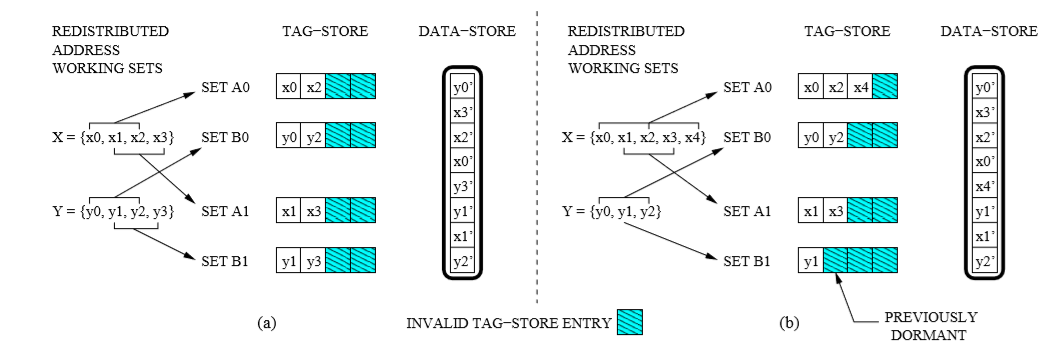
\includegraphics[width=1\textwidth]{./fig3}
\caption{ Variable-way set-associative cache using global replacement.}

\label{fig3}
\end{figure}

\newpage

\section{ V-Way Cache}
\subsection{Terminology}
Now here  property of the V-Way cache is the existence of more tag-store entries than data lines. Now defines the tag-to-data ratio (TDR) as the ratio of the number of tag-store entries to the number of data lines, where TDR ≥ 1. The case TDR = 1 is equivalent to a traditional cache. In the example in Section 2, TDR = 2 because there are twice as many tag-store entries as data lines. 

\subsection{Structure}

\begin{figure}[h!]
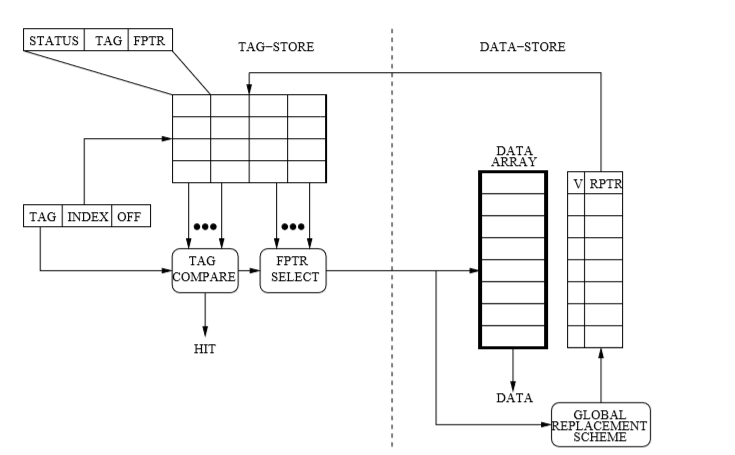
\includegraphics[width=1\textwidth]{./fig4}
\caption{  V-Way Cache.}
\label{fig4}
\end{figure}

figure \ref{fig4} is given here shows the structure of The \emph{V-way cache}. The \emph{V-way cache} has two decoupled structure: the tag-store and data-store.Each entry on the tag-store contains status information (a valid bit, dirty bit, and replacement information), tag bits and Foward Pointer(FPTR) which identifies the unique entry in data-store.

\vspace{.8cm}
If the valid bit in a tag-store entry is cleared, all  other information in the entry, including the FTPR ,is considered invalid. Each data-store entry contains a data line and valid bit a reverse pointer (RPTR). This pointer finds a unique entry in tag store. 




\subsection{ Operation}

As We know that A \emph{V-way cache} consists of two sequential array lookups, depending on whether the first lookup is performed first.If the tag-store gets a hit, the FPTR is used to perform a direct-mapped lookup into data-store to get the data line.Replacement information is updated accordingly in both.If the tag-store lookup fails to get a matching entry, a cache miss is signaled because the tag-store and data-store are decoupled, two victims must be identified for ensuing line fill: a tag-victim and a data-victim.


\vspace{.8cm}
The tag-victim is always one of the entries in the target set of tag-store and is chosen before it And selection of this is based on two scenarios:
\begin{enumerate}

\vspace{.8cm}

\item \emph{there exists a least one invalid tag-store entry in the set.}
Because there are twice as many tags as data lines, the probability of getting an invalid entry in the set is high. In $12$ out of $16$ benchmarks studies and $90\%$ victims were provided by invalided entries. The tag-victim is updated with a victim and valid set and The RPTR of data is updated to point the new one and finally, replacement information is updated to both.


\item \emph{All tag-store entires in tagte set are valid}.
It is the uncommon case given that tag-victim is chosen using the local replacement scheme of the tag-store .The tag-victim in the line case contains a valid FPTR and data lines to which it pints and bypassing the data-store is evicted from cache and a write-back is scheduled if necessary  as it already points to correct one, replacement information is updated to both

\end{enumerate}
\vspace{.8cm}

In a basic set-associative cache, after an initial period, all tag-store entries in the cache are valid and barring invalidation that already occurred due to implacement of cache coherency p protocol.In the \emph{V-way cache} each time datastore's global replacement engine is run to find a victim, tag-store entry is unlikely to be used in future is invalid.

\vspace{.8cm}
The proposed \emph{V-way cache} in figure \ref{fig4} has a maximum associativity of four ways, but the technique can apply in general to any set-associative cache.
\emph{A V-way cache} can potentially achieve better miss rate of twice its size.The success of this cache depends on how well its replacement engine chooses data-victim.

\vspace{3cm}
\section{ Designing a Practical Global Replacement Algorithm}

Here the ability of \emph{V-way cache} to reduce miss rate totally depends upon on intelligence of global replacement policy.  A policy such as  \emph{Random }or  \emph{FIFO} increases miss rate as we know that when compared against a baseline configuration (TDR=1).  \emph{Perfect LRU} is far better and more effective than this policy and has space complexity of O$(n^2)$.

\vspace{.8cm}
Here they intend to design a replacement algorithm that performs comparably to \emph{Perfact LRU} method at lower cost in both hardware and latency.

\subsection{Reuse Frequency}

The Stream of references that are accessed in the second level cache (L2) is filtered version of the main memory references stream as seen by the first level cache (L1). In other words, only those addresses that miss in L1 is transferred to L2. This filtering effect typically results in much lower of locality in L2 than L1.

They here defined \emph{reuse count} as the number of L2 access to a cache line after its initial line fill.
When the L2 line is installed it resue count is set to zero and then increased by on for each L2 access.
a line is evicted from L2 cache its reuse count is read and the bucket of global distribution is increased by one.the figure \ref{fig5} shows the distribution of resue counts for all evicted lines in L2.


\begin{figure}[h!]
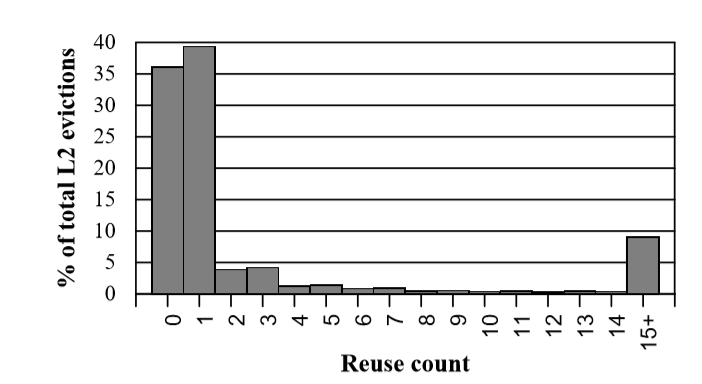
\includegraphics[width=1\textwidth]{./fig5}
\caption{ Distribution of L2 cache line reuse.}
\label{fig5}
\end{figure}

 \subsection{Cost Effectiveness of Frequency Based Replacement}

Before the research has found the significance of access frequency on relationship to cache permanence. Few author has proposed the use of frequency information for placement and replacement of cache lines. \emph{Johnson} loses frequency information to make cache bypass decision. \emph{Hallnor et al }use access frequency with hysteresis to implement an algorithm called generalization replacement, which requires $33$ bits of information per tag-store entry.

\vspace{.8cm}

\subsection{ Reuse Replacement}


Now here they are proposing \emph{Reuse Replacement}, a
frequency based global replacement algorithm that is both fast and inexpensive in terms of cost. Figure 1.6(a) shows the structure that required to implement this algorithm.
\vspace{.8cm}


Every data line in the cache has an associated reuse counter. The reuse counters are two-bit saturating counters and these are kept in \emph{Reuse Counter Table} to avoid accessing the data when reading or updating. PTR register points to entry in RCT where global replacement engine will begin searching for next victim .

\begin{figure}[h!]
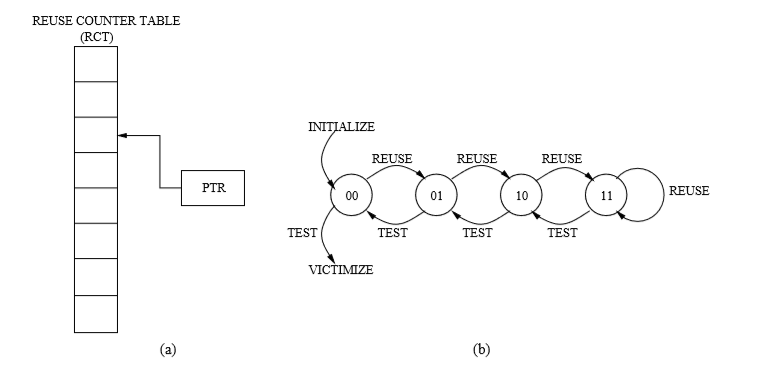
\includegraphics[width=1\textwidth]{./fig6}
\caption{Reuse Replacement : (a) RCT and PTR register. (b) State machine for the reuse counters.}
\label{fig6}
\end{figure}
When a cache line is installed in the cache, the reuse counter with the corresponding data-story entry is set to zero.For each access to a cache line, the reuse counter is increased by saturating arithmetic.On a cache miss, the global replacement engine searches the RCT for a reuse counter equal to zero.

\subsection{Variable Replacement Latency}

\vspace{1cm}
The Reuse Replacement algorithm is guaranteed to find a victim, the time required to do so can be vary depending upon the overall level of reuse in the program. They refer to \emph{victim distance} as the number of times the PTR register in increased before the victim is found.In the theoretical worst case, every reuse counter in the RCT is saturated, victim distance will have the  value $(2^N-1)$ X NUM\_REUSE\_COUNTER for an N-bit reuse counter. They expect the victim's distance to be lower than the theoretical maximum for two reasons.First of all, the majority of cache line exhibit reuse as shown in figure\ref{fig5}. Second, decoupling the tag-store entries from data-store entries has the effect of randomizing the memory access pattern generating long victim distances.


\vspace{.8cm}
Assuming that eight counters can be tested in one cycle, Table \ref{table1} Shows the probability of finding a victim as search time increases, based on experimentation.
\vspace{.8cm}
\begin{table}[h!]
\centering
\caption{Probability of finding a data-victim as replacement latency increases. }
\label{table1}
\begin{tabular}{llllll}
\hline
\multicolumn{1}{|l|}{Latency}    & \multicolumn{1}{l|}{1 cycle} & \multicolumn{1}{l|}{2 cycle} & \multicolumn{1}{l|}{3 cycle} & \multicolumn{1}{l|}{4 cycle} & \multicolumn{1}{l|}{5 cycle} \\ \hline
\multicolumn{1}{|l|}{probablity} & \multicolumn{1}{l|}{91.3\%}  & \multicolumn{1}{l|}{96.9\%}  & \multicolumn{1}{l|}{98.3\%}  & \multicolumn{1}{l|}{98.9\%}  & \multicolumn{1}{l|}{99.2\%}  \\ \hline
                                 &                              &                              &                              &                              &                              \\
                                 &                              &                              &                              &                              &                             
\end{tabular}
\end{table}

The probability of finding a victim under five cycle is $99.2\% $, and five cycles is well below the miss latency of modern secondary caches. to avoid this victim-distances, however, the global replacement engine terminates the search five cycles and use the entry pointed by the PTR as data-victim.

\section{ Results}
\subsection{Performance of V-Way Cache}
\vspace{1cm}
Figure \ref{fig7} shows us the relative miss rate reduction for three different cache configuration compared against the baseline cache. \emph{The V-way cache} has a maximum associativity of 8 ways and the both  \emph{The V-way cache} and fully associative cache have a $256$KB data-store.The third cache configuration is a basic set-associative cache with same line size and associativity as the baseline but the data-store is doubled to $512$KB.


in Figure \ref{fig7} we can see the \emph{V-way} cache approached this upper bound for \emph{perlbmk,facerec, and gcc.}They refer to primary upper bound as a \emph{loose upper bound } because differences in the \emph{LRU and Reuse Replacement} policies can result in the\emph{ V-way} cache outperforming the fully-associative cache as seen with \emph{crafty,vortex,vpr,twolf.}

\begin{figure}[t]
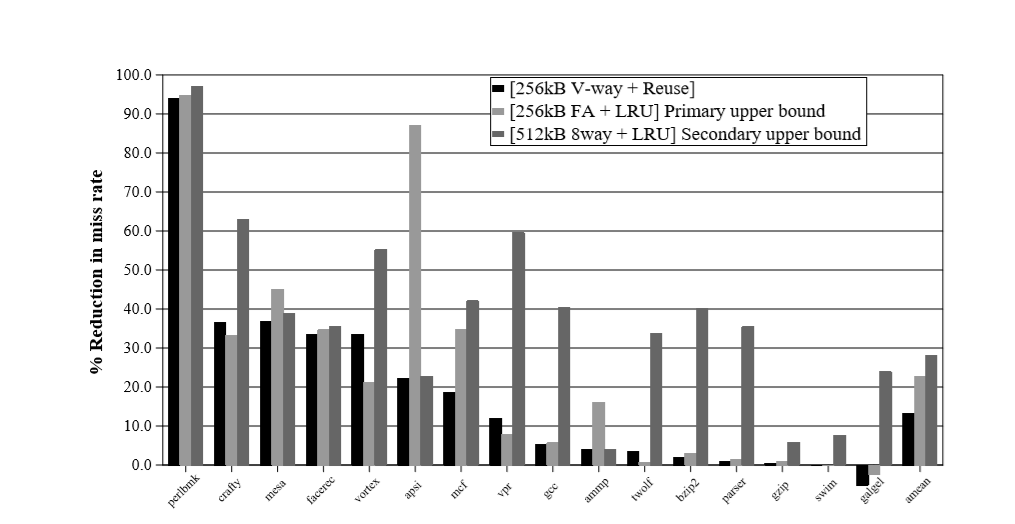
\includegraphics[width=1\textwidth]{./fig7}
\caption{Reduction in miss rate with : V-way cache (TDR=2), fully-associative cache, and double sized baseline.}
\label{fig7}
\end{figure}
\begin{figure}[h!]
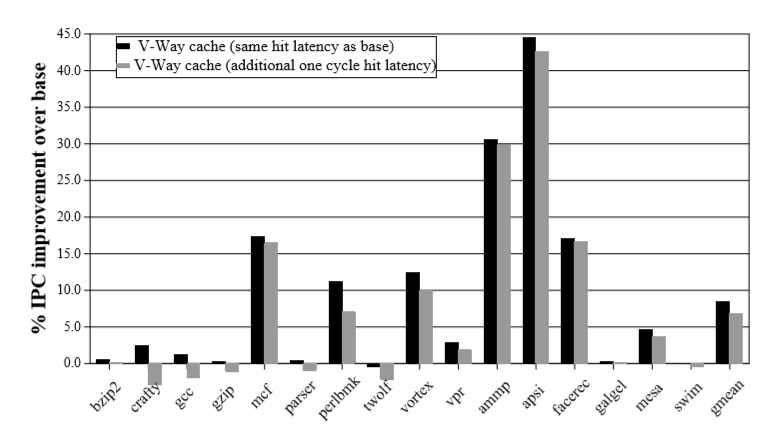
\includegraphics[width=1\textwidth]{./fig8}
\caption{ Percentage IPC improvement over the baseline for a system with a V-Way L2 cache.}
\label{fig8}
\end{figure}


\chapter{A Case for MLP-Aware Cache Replacement}
\section{Introdcution}

\vspace{.8cm}

As we know that imbalance between processor and memory speeds increases, the focus is improving the system performance over to the memory system.When there is a miss at largest on-chip cache, processing stops after a few cycle and the resources remain in the idle situation for many more cycles.The inability to process instructions in parallel with long-latency cache misses gets in performance loss.

\subsection{Not All Misses are Created Equal}


The servicing misses in parallel decreases the number of time of the processor has to stop due to given number of long-latency memory access. However, \emph{MLP} is not uniform across all the memory access in a program. Some miss occurs in isolation due to pointer-chasing loads, some misses occur in parallel; with other.the performance loss due to from a cache is reduced when multiple caches are services in parallel because the idle cycles waiting for memory to get amortized over the misses.

\vspace{.8cm}
Traditional cache replacement algorithms are not aware of the display in performance loss that results from the variation in \emph{MLP} among the cache misses. The replacement methods try to decrease the number of misses with an implicit assumption that reduction in misses correlates with the reduction in \emph{MLP}, the number of misses may or may not correlate directly with the number of cycles .

\vspace{.8cm}


\begin{figure}[h!]
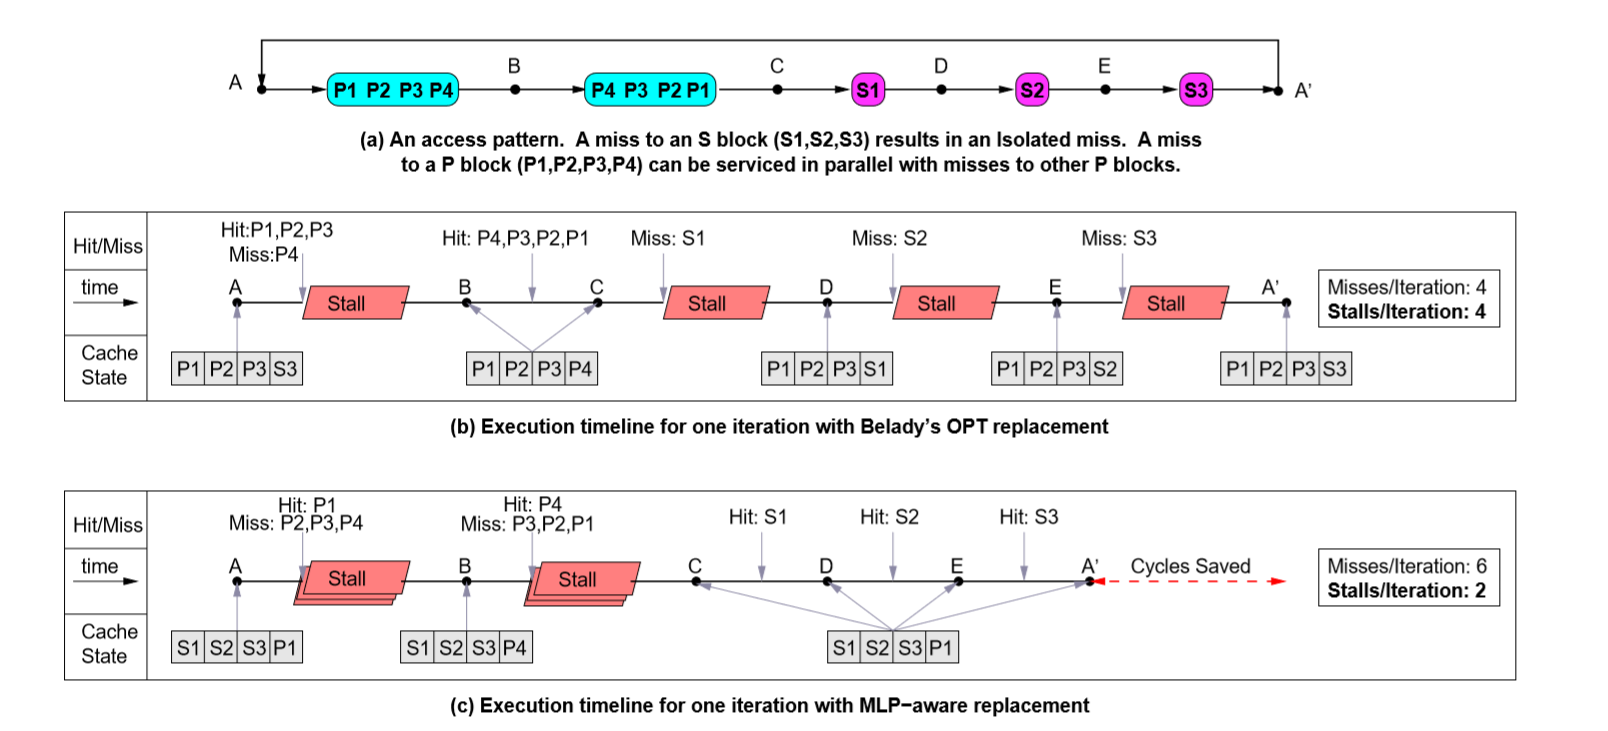
\includegraphics[width=1\textwidth]{./fig9}
\caption{ The drawback of not including MLP information in replacement decisions.}
\label{fig9}
\end{figure}

\vspace{.8cm}
 Figure \ref{fig9} (a) shows a loop containing 11 memory references. There are no other memory access instructions in the loop and the loop iterates many times. 

\vspace{.8cm}
First let us consider a replacement method which tries to minimize the number of misses, without taking \emph{MLP} information into account. \emph{Belady's OPT} provides a theoretical minimum for the number of misses by evicting a block that is going to accessed farthest in the future.
Figure 1(b) shows the behaviour of \emph{Belady's OPT} for a given the access stream. At point B, block P1, P2, P3 and P4 were accessed in the immediate past and will be accessed again in the future So the cache contains Block P1, P2, P3 andP4 at point B. This results in hits for the next access block P4, P3, P2, P1 and misses for S1, S2, S3, S4 blocks.\vspace{.8cm}



Second .consider a simple \emph{MLP-aware} Policy, which tries to reduce the number of isolate misses.This Method keeps un cache the blocks that lead to isolated misses (S1, S2, S3) rather than the blocks that lead to parallel misses (P1, P2, P3, P4). Such method evicts the least-recently-used P-block form the cache.From Figure 1(c) shows the behaviour of Such \emph{MLP-aware} policy for a given access stream. The cache has space for four blocks and the loop contains only 3 S-block (S1, S2, S3) therefore it never affects any s-bock at any point in the loop. At the first loo[ iteration each access to S1, S2, S3 gets a hit.The block P1, P2, P3 gets a miss.
\vspace{.8cm}
\subsection{ Contributions }
Based on the observation that the aims of  cache replacement policy algorithms is to reduce the memory relate stalls rather than to reduce the raw number, we propose \emph{MLP-aware} cache replacement and make the following contributions;
\begin{enumerate}
\item As a first step to enable \emph{MLP-aware} cache replacement, they propose run-time algorithms that can compute a cost for in-flight misses.
\item they show that for most benchmark .\emph{MLP-aware} cost for misses to individual cache blocks. The last time \emph{MLP-aware} cost can be used as  a predictor for next time \emph{MLP-aware} cost.

\item They propose a simple replacement policy called Linear policy (LIN) which takes both recency and \emph{MLP-aware} cost into account to implement a practical \emph{MLP-aware} cache replacement method. This shows a  $23\%$ improvement with policy in becnhmarks.

\item The LIN policy does not perform well for the benchmark in which the \emph{MLP-based} cost differs for misses to an individual cache block. They proposed the \emph{Tournament Selection(TSEL)} method to selects between \emph{LIN } and \emph{ LRU} on per-set basis, depending on which policy results in the least number of memory-related stall cycles

\item It is expensive to implement to a \emph{TSEL} method on a per-set basis for all the set in the cache . Based on the key in-sight that a few sampled set can be used to decide the replacement policy globally for the care they proposed a method called which is a \emph{low-hardware Adaptive Replacement(SBAR) } .\emph{SBAR} allows dynamic selection between \emph{LIN} and \emph{LRU} while incurring a storage overhead of 1885B.

\end{enumerate}

\section{Background}


Out-of-order execution inherently improves \emph{MLP}
by continuing the execute instruction after a long-latency miss. Instruction processing stops only when the instruction window becomes full.The analytical model of out-of-order superscalar processor proposed by \emph{Karkhanis} and \emph{Smith} provides fundamental insight into how parallelism in L2 missed can reduce the cycles per instruction incurred due to L2 misses.\vspace{.8cm}


The effectiveness of an out of order going ability to increase  \emph {MLP} is limited by the instruction windows size. Several proposals have looked at the problem of scaling the instruction window for out of order processor.They concluded that microarchitecture optimization can have the profound impact on increasing \emph{MLP}. They also formally defined instantaneous \emph{MLP}  as \emph{ the number if useful long-latency off-chip accesses outstanding when there is at least one such access outstanding.}


All of the techniques which are describes thus so far by them here is try to improve \emph{MLP} by overlapping long-latency memory operations. \emph{MLP} is not uniform across all memory access in a program. While some of the misses are parallelized many misses still occur in isolation IT makes sense to make this variation in \emph{MLP} visible to the cache replacement algorithms. cache replacement if made \emph{MLP-aware} can increase performance reducing the number of isolated misses at expense of parallel misses. Critically, as defined, is determined by how long instruction processing continues after load miss n where \emph{MLP} is determined by how many additional misses are encounter while servicing a miss.In general, any cost-based replacement method including the one which is proposed here can be used for implementing a \emph{MLP-aware} replacement policy. However to use any cost-based replacement method they first need to define the cost of each block based on the \emph{MLP} with which it was serviced. As the first step to enable MLP-aware cache replacement, they introduce a run-time method to compute \emph{MLP-based} cost.


\section{ Computing MLP-Based Cost}


For  current instruction for the window sizes, instruction processing stalls shortly after a long-latency miss occurs. The number of cycles for which a miss stalls the processor can be approximated by the number of cycles that the miss spends waiting to get serviced. For parallel misses, the stall cycles can be divided equally among all concurrent misses.


\subsection{ Algorithm}

The information about the number of in-flight misses that we need and the number of cycles a miss is waiting to get serviced can easily be tracked by \emph{MSHR}
(Miss Status Holding Register). Each miss is allocated a
\emph{MSHR} entry before a request to services that miss is to sent memory. To compute The \emph{MLP-based} cost they add a filed \emph{$mlp\_cost$} to each
\emph{MSHR} entry.
\begin{figure}[h!]
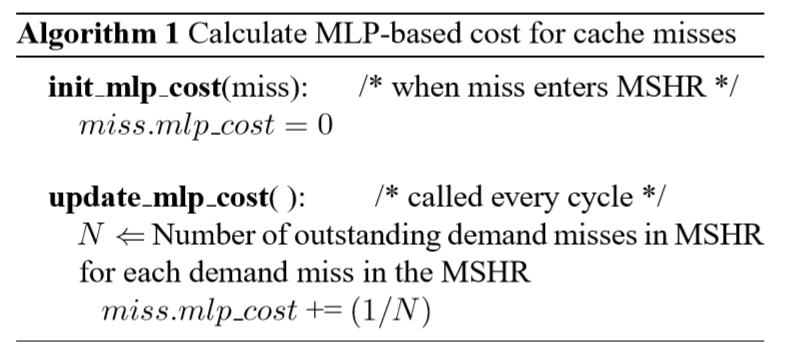
\includegraphics[width=1\textwidth]{./fig10}

\end{figure}

When a miss is allocated a \emph{MSHR} entry. the $mlp\_cost$ field associated with that entry is set to 0 (zero). they count instruction access, load access and store access that miss in the largest on-chip cache as demand misses.Each cycle the $mlp\_cost$ of all misses in the \emph{MSHR} is increased by one when an is serviced the  $mlp\_cost$ filed in the \emph{MSHR} represents the \emph{MLP-based} cost of that miss.

\begin{figure}[h!]
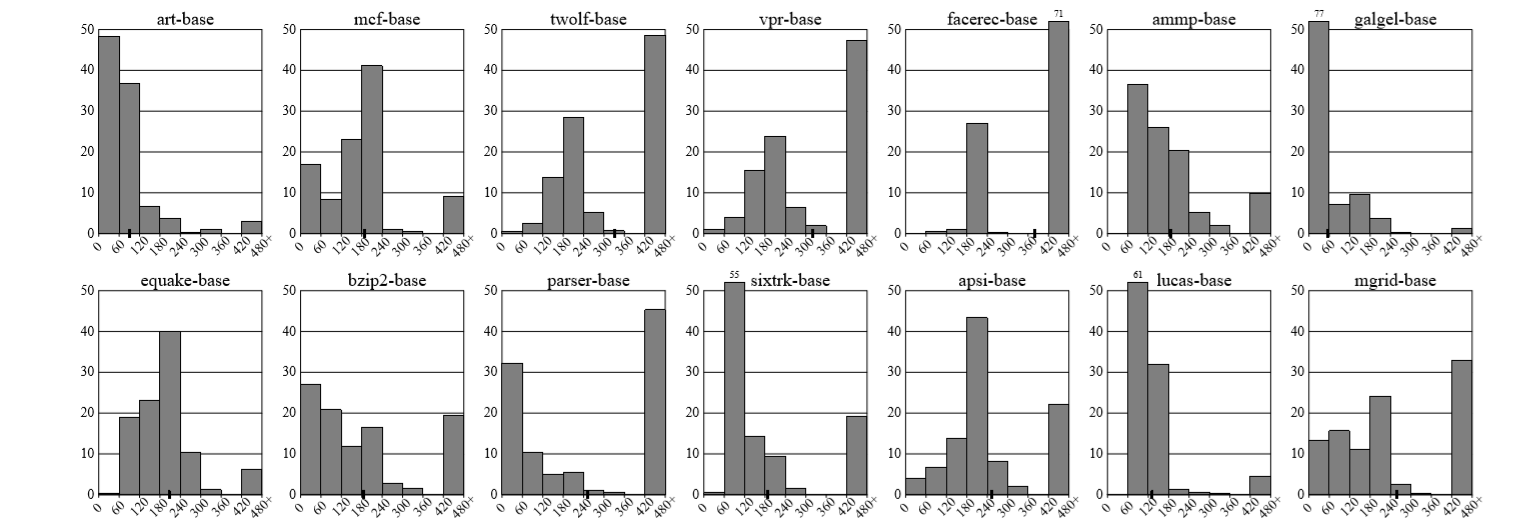
\includegraphics[width=1\textwidth]{./fig11}
\caption{Distribution of $mlp-cost$. The horizontal axis represents the value of mlp-cost in cycles and the vertical axis represents the percentage of total misses. The dot on the horizontal axis represents the average value of $mlp-cost$.}
\label{fig11}

\end{figure}

\subsection{ Distribution of $mlp-cost$}
\vspace{.8cm}

Figure \ref{fig11} shows the distribution of $mlp\_cost$ for 
14 SPEC benchmark measured on an eight-wide issue, out-of-order processor with $128$-entry instruction window. An isolated miss takes $444$ cycles to get serviced. The vertical axis represents the percentage of all misses and the horizontal axis corresponds to differ values of $mlp\_cot $. The graph is plotted with $60$-cycle intervals with the leftmost bar representing the percentage of missed that had a value of $0<=mlp\_cost<60$ cycles. The rightmost part represents the percentage of all missed that had a $mlp\_cost$ of more than $420$ cycles.For Each Benchmark, the average value of $mlp\-cost$
is much less than $444$ cycles. For art, more than $85\%$ of the misses have a $mlp\-cost$ of less than $120$ cycle indicating a high parallelism in misses. The Objective of \emph{MLP-aware} cache replacement is to reduce the number of isolated missed without substantially increasing the total misses. $mlp\-cost$ can serve as useful metric in designing an  \emph{MLP-aware} replacement method

\subsection{Predictability of the $mlp-cost$ metric}

One way to predict the future $mlp\_cost$ value of a block is to use the current  $mlp\_cost$ value of that block. The usefulness of this method can evaluate by measuring the difference between the  $mlp\_cost$ for misses which are successive to a cache block. 


We call the absolute difference in the value of  $mlp\_cost$ for misses which are successive in nature to cache block as \emph{delta}.   For example, let cache block A have $mlp\-cost$ values of {$444$ cycles, $80$ cycles, $80$ cycles, $220$ cycles} for the four misses it had in the program. Then, the first \emph{delta} for block A is $364$ (k444−80k) cycles.
\vspace{.8cm}


For all the benchmark , except \emph{bzip2,parser},and \emph{mgrid} the majority of \emph{delta} values are less than $60$ cycles. The average \emph{delta} value of also failry low which measn the next time $mlp\_cost$ for a cahce block reamins  failry close to currebt $mlp\_cost$  ths current $mlp\_cost$ can be used as predictor of the next $mlp\_cost$ of same block in \emph{MLP-aware} cache replacement .

\section{ The Design of an MLP-Aware Cache Replacement Scheme}
\vspace{.8cm}

Figure \ref{fig12}(a) shows the microarchitecture design for \emph{MLP-aware} cache replacement . The added structure are shaded. The cost calculation logic (CCl) contains the hardware implementation of Algorithms 1. It computes $mlp\-cost$ for all demand misses. When miss gets serviced, the $mlp\-cost$ of the miss is stored in tag-store of that cache blocks. For replacement, the cache invokes the \emph{Cost Aware Replacement Engine(CARE)} to find the victim. CARE can consist of any generic cost-based method. They evaluate the \emph{MLP-aware} cache replacement using both existing as well as novel cost based replacement method. 

\begin{figure}[h!]
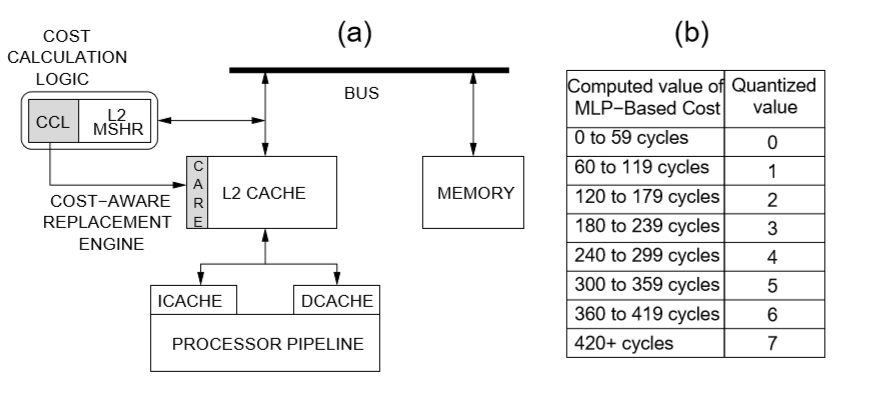
\includegraphics[width=1\textwidth]{./fig12}
\caption{ (a) Microarchitecture for MLP-aware cache replacement (Figure not to scale). (b) Quantization of $mlp-cost$.}
\label{fig12}


\end{figure}

\subsection{ The Linear (LIN) Policy}

The baseline Replacement policy is LRU so it selects the candidate of cache block with least recently. Let $Victim_{LRU}$ be the victim selected by LRU and $R(i)$ be recency.

\begin{equation}
\vspace {1cm}
          Victim_{LRU} = arg \hspace*{.6cm} min \{ R(i) \}  
\end{equation}

They want a policy that takes into account both $Cost_q$ and Recency. They propose a replacement policy that employs a linear function of recency and $cost_q$. They call it Linear (LIN) policy.

\vspace {1cm}
\begin{equation}
\vspace {1cm}
          Victim_{LRU} = arg \hspace*{.6cm} min \{ R(i) +\lambda.Cost_q(i)\}  
\end{equation}


The parameter $\lambda$ determines the importance of $Cost_q$ in choosing the replacement victim.In case of a tie for the minimum value of  $\{R+\lambda.Cost_q\}$, the candidate with smallest recency value is selected.With a high $\lambda$ value, LIN policy tries to retain recent cache blocks that have high $mlp\_cost$.

\subsection{ Results for the LIN Policy}
\begin{figure}[h!]
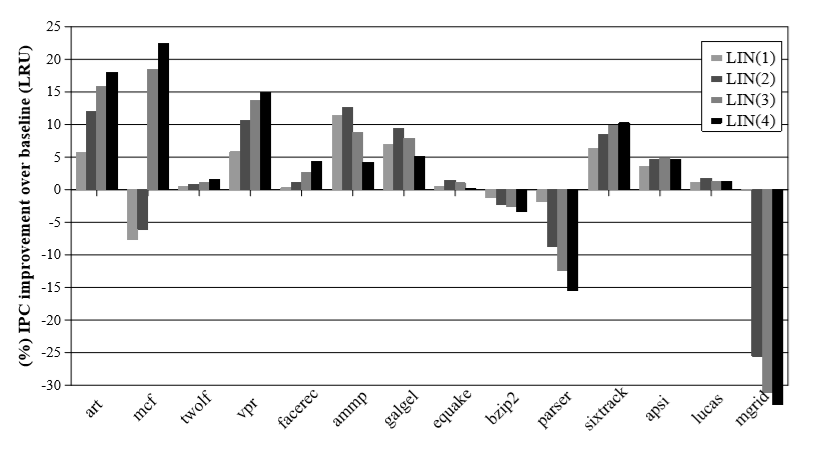
\includegraphics[width=1\textwidth]{./fig13}
\caption{ IPC improvement with LIN ($\lambda$ ) as $\lambda$ is varied.}
\label{fig13}

\end{figure}
\section{Tournament Selection of Replacement (TSEL) Policy}

Let \emph{MTD} be the main tag directory of cache. For facilitating hybrid replacement. \emph{MTD} is capable of implementing both \emph{LIN} and \emph{LRU}.\emph{MTD} is happened with two auxiliary tag directory (ATD): \emph{ATD-LIN} and \emph{ATD-LRU}. Noth has the same associativity as \emph{MTD}.  A Saturating Counter (SCTR) keep track of which of two ATDs is doing better. The access stream visible to \emph{MTD} is chosen based on the output of SCTR. They call it AS \emph{ Tournament Selection (TSEL)}. Figure \ref{fig14} shows the operation of The TSEL for one set in the cache.

\begin{figure}[h!]
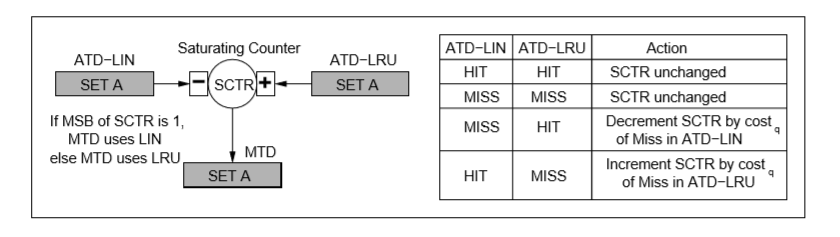
\includegraphics[width=1\textwidth]{./fig14}
\caption{Tournament Selection for a single set. }
\label{fig14}
\end{figure}

the example in Figure 7(b), sampling reduces the number of ATD entries required for the TSEL-global mechanism to 3/8 of its original value. A natural question is: how many leader sets are sufficient to select the best performing replacement policy? 


\begin{figure}[h!]
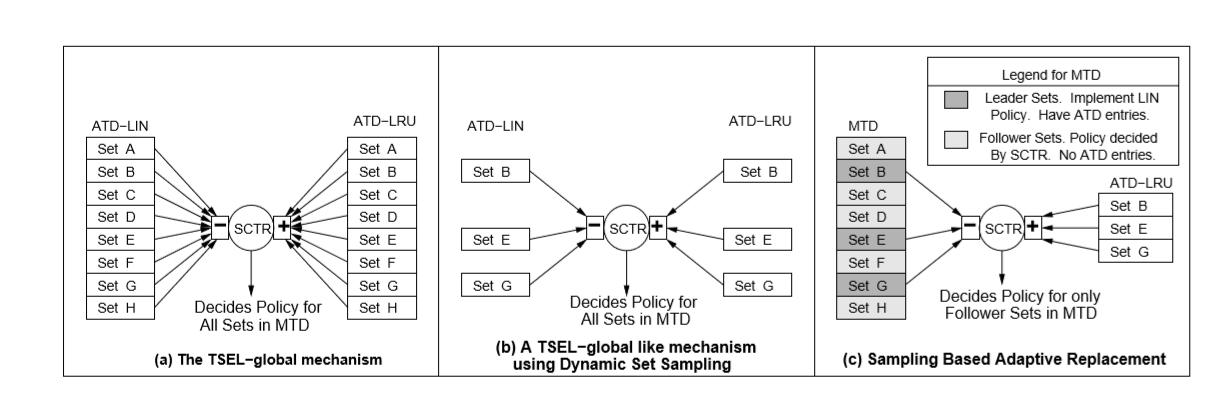
\includegraphics[width=1\textwidth]{./fig15}
\caption{ (a) The TSEL-global mechanism (b) An approximation to TSEL-global mechanism using sampling (c) Sampling Based Adaptive Replacement (SBAR) for a cache that has eight sets.}
\label{fig15}
\end{figure}

\vspace{.8cm}
\section{ Dynamic Set Sampling}
A very simple method but very expensive one is a way to implement the hybrid replacement for TSEL method for every set in the cache. In such implementation for each set in \emph{MTD} there would be a set in \emph{ATD-LIN} and \emph{ATD-LRU} and SCTR counter. \emph{MTD} can consult the SCTR corresponding to its set for choosing between LIN and LRU. 

They call this implementation TSEL-local require two ATDS each sized the same as \emph{MTD}. which makes it a high-overhead option.Another method of extending the TSEl method for the entire cache is to have both \emph{ATD-LIN} and \emph{ATD-LRU} feed a single SCTR counter. The output of single SCTR decides the policy for all set in \emph{MTD}. They call this method TSEL-Global.
An Example is shown in Figure \ref{fig15}(a)

\section{Sampling Based Adaptive Replacement}

Sampling makes it possible for us to chose the best performing policy with high probability even with very few sets in the ATD. Due to the number of; leader sets is small. The hardware overhead can be further reduced by embedding the functionality of one the ATDs in \emph{MTD}. Figure \ref{fig15}(c) shows such a sampling-based hybrid Scheme called Sampling used Adaptive Replacement (SBAR).The sets in \emph{MTD} are logically dived into two categories : \emph{Leader Sets} and \emph{Follower Sets}. The leader sets in \emph{MTD} use only LIN policy for replacement and updates SCTR counter. The followers set implement both LIN and LRU policy for replacement and use SCTR output to choose their policy.

\begin{figure}[h!]
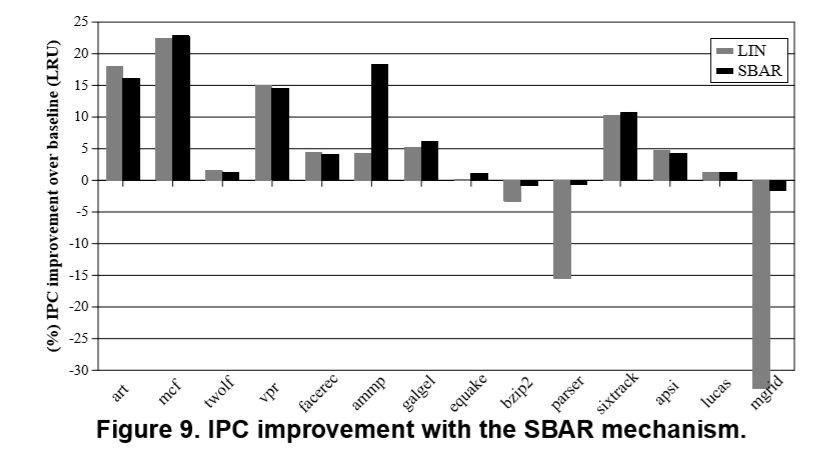
\includegraphics[width=1\textwidth]{./fig16}
\caption{ IPC improvement with the SBAR mechanism.}
\label{fig16}
\end{figure}

\section{Results}
They proposed the SBAR mechanism to implement a \emph{MLP-aware} cache replacement policy. However, the central idea of this paper, MLP-aware cache replacement, is not limited in implementation to the proposed SBAR mechanism. Our framework for MLP-aware cache replacement makes even existing cost-sensitive replacement policies applicable to the MLP domain. 

As an example, we use Adaptive Cost-Sensitive LRU (ACL)  to implement an MLP-aware replacement policy. ACL was proposed for costsensitive replacement in Non-Uniform Memory Access (NUMA) systems and used the memory access latency as the cost parameter. Similarly, MLP information about a cache block can also be used as the cost parameter in ACL. Figure \ref{fig17} shows the performance improvement of an MLP-aware replacement scheme implemented using ACL. For comparison, the results for SBAR are also shown.

\begin{figure}[h!]
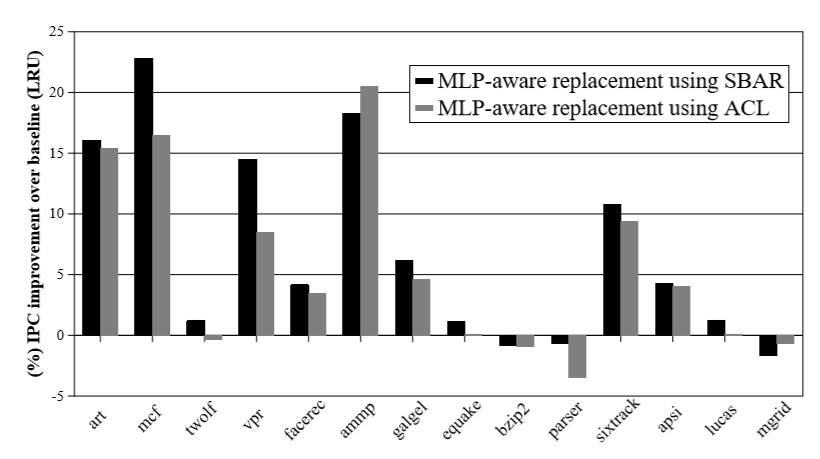
\includegraphics[width=1\textwidth]{./fig17}
\caption{  MLP-aware replacement using different costsensitive policies.}
\label{fig17}
\end{figure}

\chapter{Bank-aware Dynamic Cache Partitioning for Multicore Architectures}
\section{ INTRODUCTION }
\vspace{.5cm}
In the field of Computer architecture Chip Multiprocessors (CMP) has gradually become an attractive architecture for leveraging system integration by providing capabilities on a single die that would have previously occupied many more chip across multiple small systems which were used previously that are big in size.In a virtualization environment, workloads tend to place which are not similar demands on a shared resource and therefore due to these resource contention are much more likely to destructibility interfere in an unfair way. Consequently shared resources contention becomes the key performance bottleneck in CMPS. Shared resources include but are not limited to: Main memory bandwidth, main memory capacity, cache capacity, cache bandwidth, memory subsystem interconnection bandwidth with more system power.\vspace{.5cm}


In addition to cache partitioning need as wire delays are gradually becoming the most important design factor in the cache, architecture designers have successfully used banking techniques to migrate for increasing wire delays for the short distance. Banked architecture is now the typical design direction for caches in both industry and academia such thou are still not efficient enough since wire delay is problem. An alternative solution s the Non-Uniform Cache Architecture (NUCA) designs. NUCA is based on assuming non-uniform access latencies to all cache banks of a large L2. The NUCA model which was originally proposed for a single core was later made available for the multicore CMP version named CMP-NUCA by Beckmann et al.

So for these problems in the paper, they are contributing by proposing the following:

\begin{enumerate}
\item they propose a cache method, named \emph{Bank-aware}, for CMP-DNUCA that is aware of banking structure of L2 Cache. Thier simulation showed a $70\%$ reduction in missed compared to non-partitioned shared caches and a $25\%$ miss reduction compared to static even partitioned which is a private cache. such miss rate reduction results in overall $43\%$ and $11\%$ reduction in CPI over the non-partitioned and static even partitioned schemes respectively.

\item They demonstrate a detail implementation of dynamic cache partitioning algorithms using a non-invasive, low-overhead monitoring method based on Mattson's Stack distance algorithms. The overall hardware overhead for the proposed cache profiling method is equal to $0.4\%$ of their baseline L2 cache design.
\end{enumerate}

\section{ CMP-BASELINE }


Before this work, there are many works in industry and academia have proposed quite varied allocation and migration method for the cache memory. A large amount of work in academia has focused on free-form highly banked and non-uniform cache structures. This was in response to expected wire dominant nature of future technologies where the latency of large monolithic cache would become detrimental to the system performance.
these prosed free form caches enable great freedom in allocation and migration policies. For example, take Huh et al. proposed $256x4$ K bank cache ,in contrast industry has far typically implemented more traditional structures with fewer than eight cache bank that form multi-level  caches, for example, Intel's $45$nm Nehalem processor which is recently announced  has three level of ache ($32$KB,$256$Kb.$4-8$MB) compared to two level in previous design.\vspace{.8cm}

Figure \ref{fig18} shows their $8$-core CMP-NUCA baseline system. Their design uses as the last-level of cache a DNUCA L2 cache with$16$ physical banks that provide a total of $16$MB of cache capacity, Each of these Bank i9s configured as an $8$-way set associative cache. Another way to see the cache is as a $128$-way equivalent cache that is separated in $16$ cache banks of $8$ ways each/ The eight cache banks that are physically located next to a core called \emph{Local banks }and rest are characterized as \emph{Centre banks}.Core located next to \emph{Local banks} have minimum access latency but that dealy cab significantly increases when core need to access a \emph{Local bank} physically located next to another core. \emph{Centre banks} have on average higher access latency that n\emph{Local banks} but distance for each has smalle variation than \emph{ Local banks } so does the access latency.\vspace{.5cm}

\begin{figure}[t]
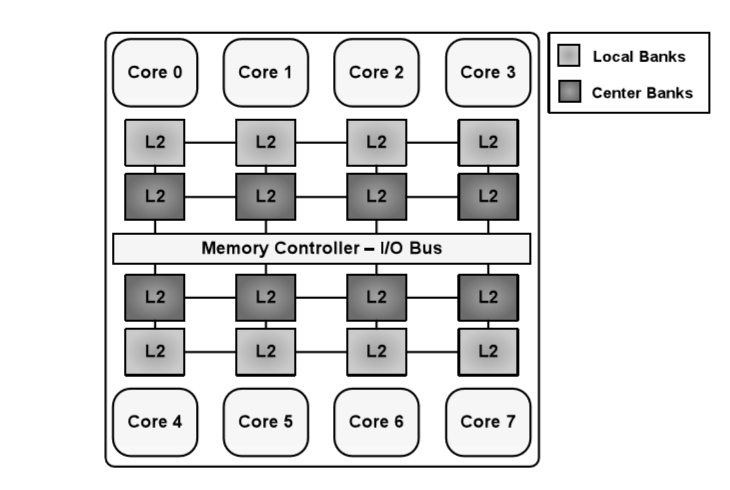
\includegraphics[width=1\textwidth]{./fig18}
\caption{  Baseline CMP system.}
\label{fig18}
\end{figure}

The maximum possible latency without significant network contention is equal to $70$ cycles(i.e. core 0 to access the \emph{Local bank} next to core $7$ since it requires $7$ hops).

\section{BANK-AWARE CACHE PARTITIONING}

The following section they elaborate on their proposed \emph{Bank-aware} cache partitioning scheme. They start by providing details about their application profiling method followed by their partition algorithms for assigning cache capacity to each core and finally, in the end, they described the cache partitioning allocation algorithm for their CMP-baseline system.

\renewcommand\thesubsection{\Alph{subsection}.}
 \subsection{Cache Profiling of Applications}
For dynamically profile the cache requirement of each core they implemented a cache miss prediction model
based on Mattson's Stack distance algorithm. Mattson's Stack algorithm was initially proposed by Matsson et al. for reducing the simulation time of trace-driven caches by determining the miss ration of all positive cache sizes with a single pass through the trace. The basic idea of the algorithm was later used for efficient trace-driven simulation of set associative cache .more recently hardware-based MSA algorithm has been proposed for CMP system resources management.


\begin{figure}[h!]
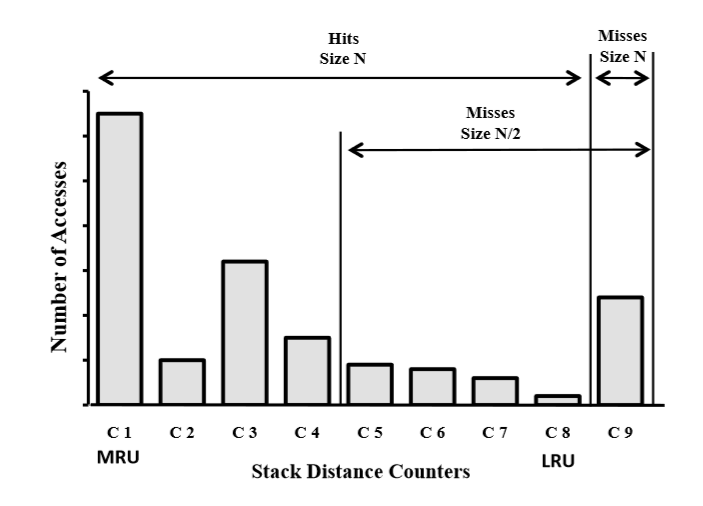
\includegraphics[width=1\textwidth]{./fig19}
\caption{    LRU histograms based on Mattson’s stack algorithm .}
\label{fig19}
\end{figure}

Figure \ref{fig19} demonstrate such MSA profile for an application running on an $8$-way associative cache. The application in the example shows a good temporal reuse of stored data in the cache the MRU position has the significant percentage of hits over the LRU position. Based on the application spatial and temporal locality the graph of Figure \ref{fig18} can change accordingly.For example, the number of misses that will occur if we make the cache of Figure \ref{fig19} half the size that is using 4 way instead of 8 ways would be previously measured misses plus the hits of the positions 5 up to 8 of the previous ache LRU stack distance. \vspace{.8cm}


Figure \ref{fig20} Shows the projected cumulative miss ration of three benchmarks of SPEC CPU2000 benchmarks suit. They selected three examples out of 26 SPEC CPU2000 workloads that they simulated as examples of varied behaviour within the whole suit. To create the figure they collected the stack distance profile of \emph{bizip2,sixtrack} and \emph{applu} with each application executing stand-alone on their baseline CMP using cache described above.


\begin{figure}[t]
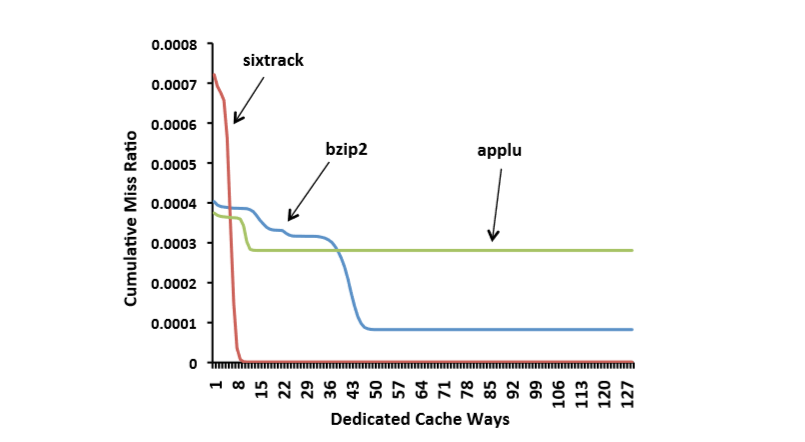
\includegraphics[width=1\textwidth]{./fig20}
\caption{    LRU histograms examples of SPEC CPU2000 benchmarks .}
\label{fig20}
\end{figure}


The x-axis represents the number of cache ways that are dedicated to each application and y-axis shows MSA-based projected cumulative miss rate f each application. \emph{Sixtrack } features a lot of miss with less than six ache ways dedicated to it but after that point, by giving more ways its misse are close to zero. \vspace{.8cm}

The hardware overhead of the profiling structure is primarily is defined by the implementation of necessary cache directory tag shadow copy. These cache blocks tags are necessary for identifying which cache block is assigned at each one of \emph{hit} counters of Figure \ref{fig19} and follow a detailed monitoring of resources requirement on ac the block granularity on their LLC.Additionally overhead is introduced by implementation of the \emph{hit} counters themselves for each cache way but since these counters are shared over all the available ache-ways there overhead is difficulty lower than the cache block tag information for every set.

% Please add the following required packages to your document preamble:
% \usepackage{graphicx}
\begin{table}[h!]
\centering
\caption{ Overhead of the proposed MSA Profiler}
\label{t1}
\resizebox{\textwidth}{!}{%
\begin{tabular}{|l|l|l|ll}
\cline{1-3}
\textbf{Structure Name} & \textbf{Overhead Equation} & \textbf{Overhead} &  &  \\ \cline{1-3}
Partial Tags & $tag\_width*ways*cache\_sets$ & 54kbits &  &  \\ \cline{1-3}
LRU Stack Distance Implem. & $((lru\_pointer\_size*ways) + head/tail)*cache\_sets$ & 27kbits &  &  \\ \cline{1-3}
Hit Counters & $cache\_ways*hit\_counter\_size$ & 2.25kbits &  &  \\ \cline{1-3}
\end{tabular}%
}
\end{table}


The hardware overhead of the proposed implementation for every necessary structure is included in Table \ref{t1}. 

 \subsection{ Bank-aware Assignment of Cache Capacity }

The work done in previously in MSA-based cache partitioning was analyzed on fully configurable cache shared among a small number of CPUs. They refer to this type of partitioning algorithm as \emph{Unrestricted}. On the other hand, while Huh et al. proposed a method for partitioning a CMP-NUCA cache this relied on a highly banked structure that as they already explained in the Section 2 feature an unrealistic physical implementation. 


\begin{figure}[t]
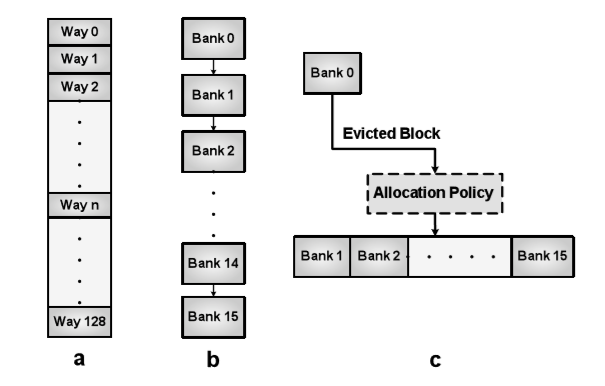
\includegraphics[width=1\textwidth]{./fig21}
\caption{   Cache banks aggregation schemes.}
\label{fig21}
\end{figure}


 As a solution, they proposed a scheme to partition cache bank structure using a MSA-based profiling method aligned with current industry directions that are using a smaller of higher capacity cache banks. Such configuration limits granularity of possible partition s and imposes a set of restrictions over the \emph{Unrestricted,} technique proposed in the past. This is rotted in the need to aggregate multiple cache bank into a single partition. I the following they discuss potential aggregation method that is shown in Figure \ref{fig21}.

Aggregation possibilities:

\begin{enumerate}

\item \textbf{Cascade:} In this approach, all cache banks that contains portion assigned to a given core are connected the head to tail. To match the MSA LRU strategy all allocation is placed as MRU at the head of the chain. Each allocation causes a shift down of LRu. Evictions are passed down to chain from LRU out of MRU position in the next bank until a free spot is located (formed from the hit hay was moved to top) Ths structure is shown in Figure b. this method proved s for an LRU policy. The advantage of this method is that one can stitch together an arbitrary fraction of banks which will emulate the MSA very closely.

\item \textbf{Address Hash:} A common approach to cache a bank aggregation is the use of a \emph{address hash}.Typically this method is used with a power of two number of cache banks such that lower order address bits can directly select the bank. While the system has also been built with non-power of two hashed this require complex modulo would be the IBM POWER4  and POWER5 processors.

\item \textbf{Parallel:} This method is very much like one given above, except that a line can be stored in any of cache banks. Allocation is controlled by round-robin selection. A such any given line can be found in any of the cache banks. This forces additional look-up operations in a directory structure. This is less restrictive than \emph{Address hash} in bank configuration. The migration rate is equivalent to \emph{Address hash} however power is higher due to wider directory look-ups.

\end{enumerate}


Based on this observation and the bank aggregation requirement they propose the following policies:
\begin{enumerate}
\item \emph{Center} cache banks are completely assigned to a specific core. This prevents situations where aggregated banks are of different capacities. 

\item  Any core that is allocated \emph{Center} banks, will receive a full\emph{ Local} bank. 

\item \emph{Local} cache banks can only be shared with an adjacent core. We only allow per assignment control at \emph{Local} cache banks.

\end{enumerate}

\vspace{.8cm}
A typical allocation is shown in Figure \ref{fig22} from the figure most of the core has multiple L2 cache banks allocated to them except L2 bank with core 3 and core 4, respectively.

\begin{figure}[h!]
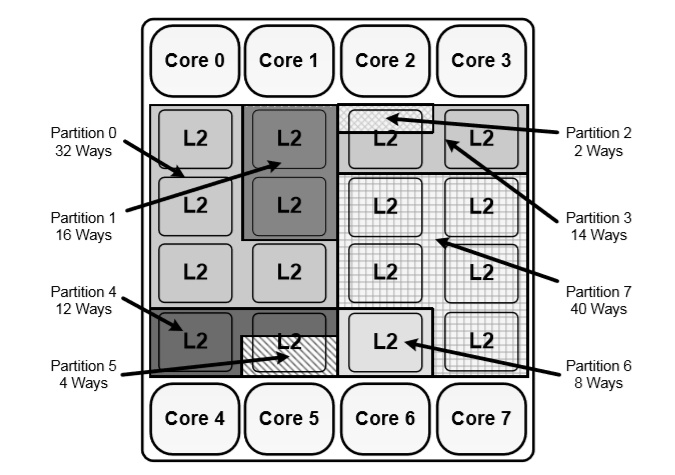
\includegraphics[width=1\textwidth]{./fig22}
\caption{ An example of typical CMP cache partitioning.}
\label{fig22}
\end{figure}


To enforce the selected cache partitions they modify the typical design of a cache bak to support a vertical fine-grain cache -way partitioning method as they proposed. According to this method, each cache-way of a set associative cache cab belong to one or more specific cores. When a specific core suffers cache miss a modified LRU policy is used to select the least recently used cache block among the ones that belong to that specific core for replacement.\vspace{.8cm}

To reduce the design complexity all of the set in cache bank is vertically partitioning with the same cache-way assigned therefore the granularity  assigning a different cache-way partition is a single cache bank.

\subsection{Allocation Algorithm on CMP}

In this section they describe in detail their \emph{Bank-aware} assignment algorithm. They uses the concept of \emph{Marginal Utility}. The amount of utility relative to the resource is defined as the \emph{Marginal Utility}. Specifically \emph{Marginal Utility} is defined as:\vspace{.8cm}
 
$$MarginalUtility(n) = MissRate(c+n)-MissRate(c)/n$$
\vspace{.8cm}


They use this capability to make the best use of limited cache resources. They follow an interative approach where at any point they can compare the \emph{Marginal Utility} of all possible allocation of unused capacity.\vspace{.8cm}

Their algorithms arrive at a capacity assignment vai success steps determining the maximum  \emph{Marginal Utility} for a subset of processors and assignment restriction.The overall flow is shown in Figure \ref{fig23}. The first step is to assign each-way in \emph{Center} cache banks.In Box 2 they check if all banks are assigned if not step 1 is repeated following Rule 1 And 2 they mark all processor with \emph{Centre} banks Complete (Box 3). In Box 4 they once again find the maximum \emph{Marginal Utility} but assigned are limited to a possible pair of the processor.\vspace{.8cm}

 In Box 5 they check of the new signage has caused any processor to overflow into another processor  \emph{Local} region if so they find the ideal pair with respect to minimum misses, Essentially we Defer the pairing as many steps as possible and make the best pairing choice once it  is decided a processor should receive a fraction of an adjacent \emph{Local bank} .Once the pair is assigned both processes are marked complete  . This step is repeated until all cache  way is assigned.
\begin{figure}[h!]
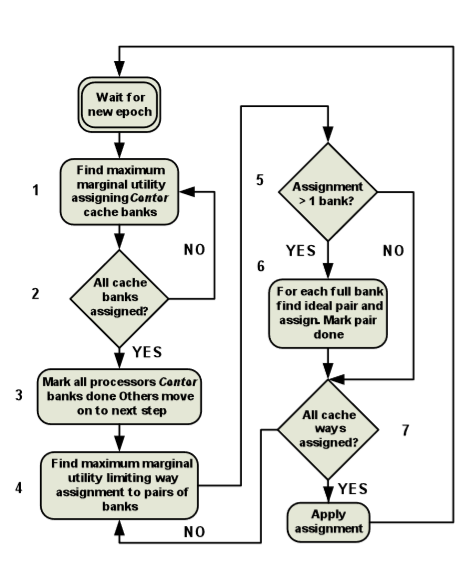
\includegraphics[width=.8\textwidth]{./fig23}
\caption{Cache allocation algorithm flow chart.}
\label{fig23}
\end{figure}

They use SPEC CPU2000  scientific benchmark suite, compiled to SPARC ISA with peak configurations, as the workload of our proposed scheme. We fast forward all the benchmarks for 1 billion instructions, and use the next 100M instructions to warm up the CMP-NUCA L2 cache. Each benchmark was simulated in our CMP-NUCA using Gems for a slice of 200M instructions after cache warm up.\vspace{2cm}



 \section{Results}
\vspace{1cm}
They randomly chose eight workload sets from the previous simulation to evaluate the proposed partitioning method on the $8$-core full system shows the selected workload along with the cache-way that were assigned to each core by \emph{Bank-aware} partition method.\vspace{.8cm}

Figure \ref{fig24} and  \ref{fig25} shows the relative miss rate and CPI of \emph{Equal-partition}. \emph{Equal-partition}. is equivalent to assigning private cache partition of equal size to each core. From the figures both partitioning schemes shows a significant reduction in misses and CPI over the simple No-partition one, which is a strong indication of the need for partition the last level of cache.
\vspace{2cm}
\begin{figure}[h!]
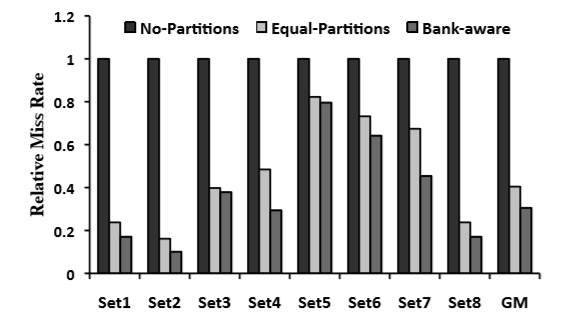
\includegraphics[width=1\textwidth]{./fig24}
\caption{  Relative miss rate of $8$-core sets over the no-partitioning scheme .}
\label{fig24}
\end{figure}
\vspace{2.5cm}


On average \emph{Bank-aware} shows a $70\%$ and $43\%$ reduction in misses and CPI over No-partition, respectively. Moreover from Figure \ref{fig24} their
 \emph{Bank-aware}  partitioning method  show on average a $25\%$ reduction over simple \emph{Equal-partition}.This reduction is inline with the direction estimated in the experiment.\vspace{.8cm}

\begin{figure}[h!]
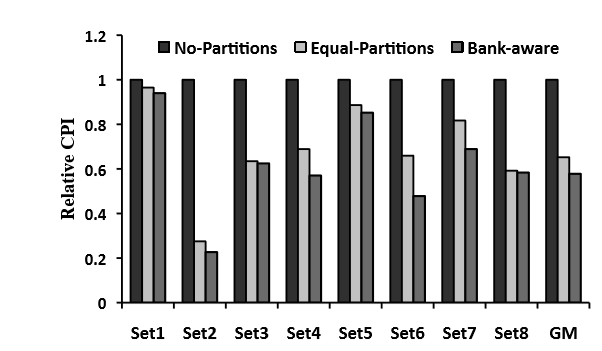
\includegraphics[width=1\textwidth]{./fig25}
\caption{ Relative CPI of 8-core sets over the no-partitioning scheme.}
\label{fig25}
\end{figure}
\vspace{.8cm}

Figure \ref{fig25} shows that their  \emph{Bank-aware}  partitioning ,method can achieve $11\%$ reduction in CPI over \emph{Equal-partition}. method. Comparing Figure \ref{fig24} and \ref{fig25} some sets of workload demonstrate a much higher performance sensitivity to missed than other since reduction on L2 misses does not always result on an equal size  reduction in CPI.

\chapter{Conclusion}

We have studied the three research papers in the field of cache memory: \textit{The V-Way Cache: Demand-Based Associativity via Global Replacement}
  \cite{Qureshi2005TheVC}\textit{A Case for MLP-Aware Cache Replacement}\cite{Qureshi2006ACF} and \textit{Bank-aware Dynamic Cache Partitioning for Multicore Architectures} \cite{Kaseridis2009BankawareDC} . \vspace{.8cm}

The V way cache provides a platform for other optimisation such as cache compression and power management. Invalid tag-store entries can be used to maintain inclusion information without the need for duplicating cache lines in the data-store.The V-Way cache has a built-in shadow directory that can provide feedback information to the replacement policy. \vspace{.8cm}

Memory Level Parallelism (MLP) varies across different misses of an application, causing some misses to be more costly on performance than others. The non-uniformity in the performance impact of cache misses can be exposed to cache replacement policy so that it can improve performance by reducing the costly misses. \vspace{.8cm}

Shared resources contention in CMP platform has been identified as key performance bottleneck that is expected to become worse as the number of cores on a chip continues to scale to higher numbers.Many solutions have been proposed but most assume either simplified cache hierarchies with no restriction or complex cache scheme that are difficult to integrate into a real design.


\newpage


\bibliography{report} 
\bibliographystyle{ieeetr}





\end{document}
